 \section{Conference Program}

% Request review from Katy Huff
\subsection{Potential Speakers}

\subsubsection{Rita Baranwal, DOE Nuclear Energy}

\begin{minipage}{0.25\textwidth}
	\centering
	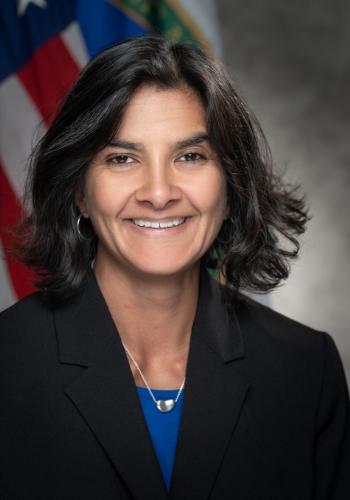
\includegraphics[width=\textwidth]{fmt-baranwal.jpg}
\end{minipage}
\begin{minipage}{0.73\textwidth}
	Dr. Rita Baranwal serves as the Assistant Secretary for the Office of Nuclear Energy in the U.S. Department of Energy (DOE).  Dr. Baranwal leads the office’s efforts to promote research and development (R$\&$D) on existing and advanced nuclear technologies that sustain the existing U.S. fleet of nuclear reactors, enable the deployment of advanced nuclear energy systems, and enhance the U.S.A.'s global commercial nuclear energy competitiveness. Prior to her current role, Dr. Baranwal directed the Gateway for Accelerated Innovation in Nuclear (GAIN) initiative at Idaho National Laboratory.  She was responsible for providing the nuclear industry and other stakeholders access to DOE's state-of-the-art R$\&$D expertise, capabilities, and infrastructure to achieve faster and cost-effective development, demonstration, and ultimate deployment of innovative nuclear energy technologies. Under her leadership, GAIN positively impacted over 120 companies. Baranwal is a clear choice of speaker to discuss the ways to improve nuclear legislation and how companies can rapidly develop new nuclear technology.
\end{minipage}

\subsubsection{Rachel Slaybaugh, UC Berkeley}
\begin{minipage}{0.25\textwidth}
	\centering
	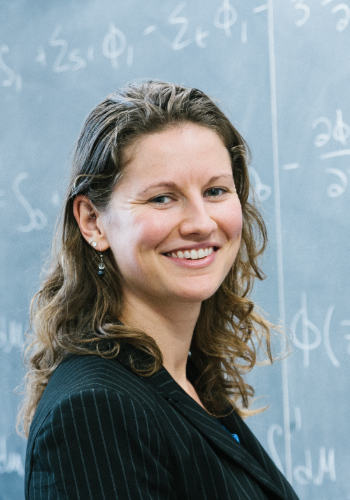
\includegraphics[width=\textwidth]{fmt-slaybaugh.jpg}
\end{minipage}
\begin{minipage}{0.73\textwidth}
	Prof. Slaybaugh's research is based in numerical methods for neutron transport with an emphasis on supercomputing. She applies these methods to reactor design, shielding, and nuclear security and nonproliferation. Slaybaugh was a key founder of the nuclear innovation bootcamp, which seeks to train students and professionals in skills essential to innovation in nuclear energy while executing team projects. Finally, Slaybaugh has served as a Program Director at ARPA-E, developing and running their first fission energy programs. Advanced Research Projects Agency-Energy (ARPA-E) invests in research for ways to generate, use, and store energy. These projects have the potential to radically improve economic prosperity in the U.S. and environmental wellbeing. Due to her endeavors in teaching and sharing nuclear innovation, we believe that Slaybaugh's goals are aligned with the goals of this conference and would make her an excellent addition to the program. Slaybaugh has much to offer the conference with her vision and leadership.
\end{minipage}

\subsubsection{William Magwood}
\begin{minipage}{0.25\textwidth}
	\centering
	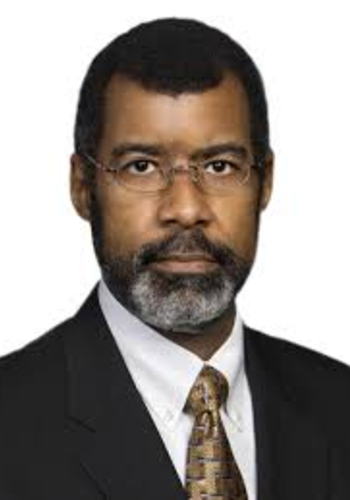
\includegraphics[width=\textwidth]{fmt-magwood.jpeg}
\end{minipage}
\begin{minipage}{0.73\textwidth}
	Mr. Magwood served seven years as the Director of Nuclear Energy with the U.S. Department of Energy (DOE), where he was the senior nuclear technology official in the United States Government. He oversaw the restoration of the Federal nuclear technology program and led the creation of ``Nuclear Power 2010,'' ``Generation IV,'' and other innovative initiatives—including successful efforts that helped reverse the decline in American nuclear technology education. Since joining the NRC, he has continued his advocacy for both U.S. science and technology education and strong international cooperation. He has also sought to assure transparency and improve the agency's openness to public participation. As an NRC Commissioner, Mr. Magwood has been a strong defender of the NRC's regulatory independence and adherence to the principle that regulations should be based firmly on scientific and technical facts. From his nomination as a Commissioner, Mr. Magwood has remained committed to his promise to carry out his responsibilities ``in a manner that earns the public's trust, and always doing the right thing even when the right thing isn't easy.''
\end{minipage}

\subsubsection{Phi Nguyen, Former Vice President and Director of Engineering at Intel}
\begin{minipage}{0.25\textwidth}
	\centering
	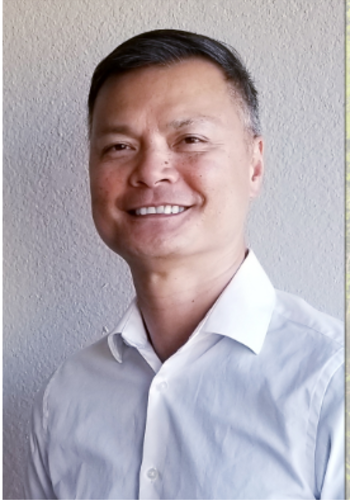
\includegraphics[width=\textwidth]{fmt-nguyen.png}
\end{minipage}
\begin{minipage}{0.73\textwidth}
Phi Nguyen, is a UIUC alumni from the NPRE department and went on to a major leadership role at the Intel corporation. Smartphones, computers, and other technology that most Americans take for granted everyday would not be possible without innovations from companies like Intel. Plasma processing plays a significant role in the production of key components of these devices. As the former Director of Engineering at Intel, Phi Nguyen is the perfect person to talk about how this important research helps solve big problems. 
	
\end{minipage}

\subsubsection{Suzanne Hobbs Baker}
\begin{minipage}{0.25\textwidth}
	\centering
	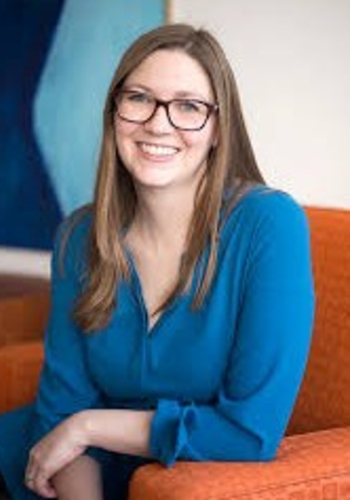
\includegraphics[width=\textwidth]{fmt-baker.jpeg}
\end{minipage}
\begin{minipage}{0.73\textwidth}
	Talking about nuclear energy, specifically with the general public, is one of Suzanne Hobbs Baker's key goals. Baker has a strong track record as a nuclear science communicator. In 2008 she founded a nonprofit organization aimed at reaching women, minorities, and young people with critical information about climate change and nuclear energy. She currently works as the creative director for Fast Path to Zero Initiatve at the University of Michigan and as a Nuclear security fellow with Third Way Energy. Baker's work in empowering minorities and students to solve the world climate crisis with nuclear energy, as well as her skill in creative science communication, ensures that Baker has a lot to offer the student conference. Celebrating the people behind the science is one of the key goals of this conference and an area in which Baker has a lot of experience.
\end{minipage}

\subsubsection{Cathy McCarthy, Canadian Nuclear Laboratories}
\begin{minipage}{0.25\textwidth}
	\centering
	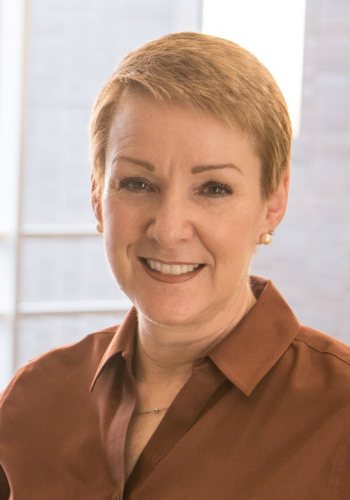
\includegraphics[width=\textwidth]{fmt-mccarthy.jpg}
\end{minipage}
\begin{minipage}{0.73\textwidth}
	Dr. Kathy McCarthy joined CNL as the Vice-President of Research and Development in 2017. Kathy has also held the position of Director of the US Department of Energy Light Water Reactor Sustainability Program Technical Integration Office. Her team, made up of scientists and engineers from across the US, conducted and guided important research that enabled power companies to be able to make informed decisions regarding long-term operation broadly, and second licence renewal specifically, for their operating nuclear units. Her expertise, leadership and contributions to the nuclear science and technology community are globally recognized, having received the American Nuclear Society Presidential Citation (2015, 2007), and the Partnership for Science \& Technology Nuclear Energy Advocate of the Year Award (2011), among many others. Her many contributions to the nuclear industry indicate that she would make a great speaker at this confrence. 
\end{minipage}


% \clearpage
\subsubsection{Jim Conca, Forbes}
\begin{minipage}{0.25\textwidth}
	\centering
	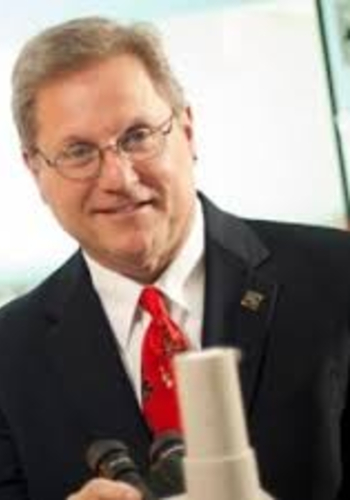
\includegraphics[width=\textwidth]{fmt-conca.jpeg}
\end{minipage}
\begin{minipage}{0.73\textwidth}
	Jim Conca has been a scientist in the field of the earth and environmental sciences for 33 years, specializing in geologic disposal of nuclear waste, energy-related research, planetary surface processes, radiobiology and shielding for space colonies, subsurface transport and environmental clean-up of heavy metals. He is a Trustee of the Herbert M. Parker Foundation, Adjunct at WSU, an Affiliate Scientist at LANL and consult on strategic planning for the DOE, EPA/State environmental agencies, and industry including companies that own nuclear, hydro, wind farms, large solar arrays, coal and gas plants. He also writes for Forbes magazine about nuclear issues, energy, and the environment. Conca has a strong vision for the future and is not shy about coming up with ideas to solve grand challenge problems. In addition to his experience and ambition, he is an excellent science communicator to scientists and non-scientists alike. Together, these factors make him an ideal speaker at the conference.
\end{minipage}


% % \clearpage
% \subsubsection{Ross Radel, CEO Phoenix, LLC}
% \begin{minipage}{0.25\textwidth}
% 	\centering
% 	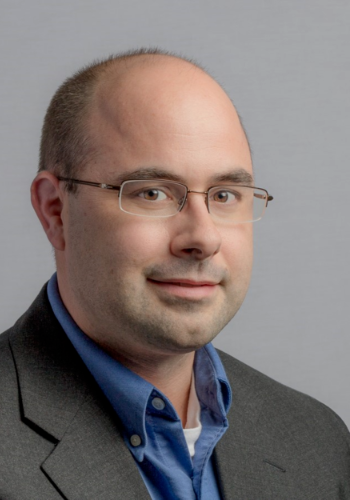
\includegraphics[width=\textwidth]{fmt-radel.png}
% \end{minipage}
% \begin{minipage}{0.73\textwidth}
% 	Ross Radel is the CEO and a Board of Directors member of Phoenix. He holds a MS and a PhD in Nuclear Engineering from the University of Wisconsin-Madison. He previously worked as the Senior Member of the Technical Staff at Sandia National Laboratories. Ross has extensive experience with nuclear reactors and advanced power conversion systems that are directly applicable to Phoenix’s core technologies. His previous research at the University of Wisconsin focused on high-flux neutron generation for detecting clandestine material, specifically highly enriched uranium. The mission of Radel's company, Phoenix, is to transform nuclear technology to better our world. This mission statement reflects our mission in hosting the student conference well. We believe Dr. Radel would be a great speaker for the future of nuclear technology.
% \end{minipage}


\subsubsection{Greg Piefer, CEO SHINE}
\begin{minipage}{0.25\textwidth}
	\centering
	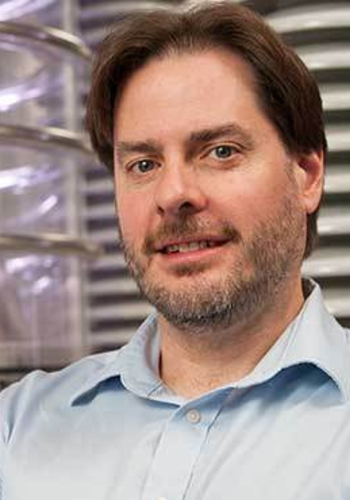
\includegraphics[width=\textwidth]{fmt-piefer.jpg}
\end{minipage}
\begin{minipage}{0.73\textwidth}
	Dr. Piefer is the founder and CEO of SHINE Medical Technologies. The mission of SHINE is to lead the world in safe, clean, and affordable production of medical tracers and treatment elements. He holds a PhD in nuclear engineering, and BS degrees in physics and electrical and computer engineering from the University of Wisconsin–Madison. Greg has received numerous awards and honors including the prestigious UW-Madison Early Career award, is the primary inventor on multiple patents and author or co-author of numerous publications, and serves on the boards of several profit and non-profit entities. His passion is the growth of technology companies that take scientific advancement to commercialization, providing the opportunity to serve and better humanity. Piefer's goals are perfectly attuned to the goals of this conference and he would be an excellent speaker on the powerful applications of radiological engineering.
\end{minipage}


\subsection{Saving the World Panel Series}
Technical and non-technical panels encourage interaction between students and professionals at the conference. Each panel is designed to address one or more of the stated goals for the conference. They also serve as a way for students and professionals to learn more about relevant issues, find inspiration for their next project, and feel encouraged for the future of the nuclear field.\\
 
$\Large\textbf{Technical Panels}$

\subsubsection{Critical Conversations: Microreactors}
Microreactors are a growing area of nuclear research and the first installations have been projected for some time in the mid 2020s. They are capable of generating 1-50 MWth, which can be used directly or converted to electricity. These relatively portable reactors are capable of powering remote areas and towns with little infrastructure. UIUC has stated that it aims to be carbon neutral by 2050. The University is exploring the possibility of constructing a microreactor on campus for research and power generation, a first of its kind, in pursuit of its decarbonization goals. This panel will discuss the benefits and applications for microreactors around the world and also talk specifically about the potential market for microreactors on universities. We have a several groups on campus researching, simulating, and modelling microreactors. Faculty leading these groups would be excellent speakers on this panel.


\subsubsection{Plasma Processing in Your Pocket}
Plasma processing has become a staple in many fields of advanced manufacturing. Without plasma, modern conveniences such as smartphones and powerful computer technology would not be possible. In this panel, representatives from companies at the cutting-edge of plasma processing research will discuss how plasmas continue to revolutionize contemporary industry. Potential panelists include Brian Jurczyk, CEO of Starfire Industries, and Phi Nguyen, former Vice President and Director of Engineering at Intel Corp.

\subsubsection{Fusion: Materials for the Future}
Nuclear fusion has the potential to serve as the ultimate clean energy source, capable of supplying the world’s energy needs for millennia. Harnessing this immensely powerful energy resource requires further innovation in a variety of scientific disciplines. One of the largest remaining obstacles to fusion energy is the unprecedented strain placed on the materials from which fusion reactors are built. This panel will focus on the latest advancements in plasma facing components research and could feature panelists such as Professor David Ruzic, director of the UIUC Center for Plasma-Material Interactions, and Dr. Lauren Garrison, Weinberg Fellow at ORNL.

\subsubsection{Nuclear Policy and Legislation}
Nuclear energy is one of the most heavily regulated fields in the United States. This panel aims to enlighten attendees about how legislation is written and how non-scientist government officials might better understand the potential of nuclear energy. This panel will allow attendees to learn who is working in this area and develop a network of people devoted to issues of nuclear policy.
Rita Baranwal would be an excellent speaker on this panel because of her work for the DOE.

\subsubsection{Radiological Techonology for a Healthier and Safer Future}
From the production of medical isotopes to nuclear verification, radiological engineering will play an important role in the future of health, security, and more. This panel will illuminate some of those applications and show attendees what could be possible with radiological technology. Speakers may include Greg Piefer from SHINE and Ross Radel from Phoenix.\\

$\Large\textbf{Non-Technical Panels}$

\subsubsection{Science is People: Conducting Inclusive Research}
Research and technology that will help us solve the grand challenge problems of the world must also reflect the diverse needs of the people that live in it. Everyone comes to nuclear engineering from a variety of backgrounds, identities, abilities, and experiences. Saving the World One Atom at a Time means making atomic contributions. Finding ways to encourage and include even one more person in the endeavor of nuclear science is an important kind of atomic contribution. This panel works toward the goal of celebrating the people behind the science. It also serves to inspire students and 

\subsubsection{Talking To Non-Scientists}
It has been shown that when members of the general public are given more scientific evidence they are less likely to shift their beliefs. While this finding is surprising to members of the scientific community, people who value data and evidence, it can be difficult to find ways to effectively communicate your research to the public. Attendees will learn how other scientists effectively communicate their results. No longer discouraged by potential resistance from the public, students will steel their resolve for working on ambitious projects that can save the world. Suzanne Hobbs Baker would be a great choice for this panel, as well as members of The Story Collider; a non-profit organization devoted to helping scientists tell stories that 

\subsubsection{How to Host a Conference}
This panel is devoted to sharing the experience of this conference's planning committee with students from other schools that may want to host their own student conference. This panel is for students by students. We will discuss our process from writing a successful proposal to executing a successful conference. 


\subsection{Workshops}

\subsubsection{Scientific Storytelling}
Science is people. The Story Collider is a non-profit organization whose mission is to honor the people and stories behind the science and teach scientists to use these stories to their advantage. From their website:
\begin{quote}
	We know that storytelling is not typically taught during scientific training, and is sometimes explicitly discouraged. There are many reasons why. But like it or not, stories are how people understand the world, and they weave together fact and emotion. Compared to other forms of communication, these narratives can be more successful in:
	\begin{itemize}
		\item generating interest and engagement with a topic,
		\item improving comprehension, and
		\item influencing real-world beliefs, even among skeptical audiences.
	\end{itemize}
\end{quote}

\subsubsection{Building Your Network}
The AAAS conducts workshops that teach early career scientists and students how to develop a professional network that will benefit them in the future. They hold regular workshops about strategic networking, making new contacts, and getting the most out of a conference. We will invite them to conduct a workshop where attendees can come away with skills to maximize their experience at the ANS Student Conference.

\subsubsection{MOOSE Workshop}
The Multiphysics Object Oriented Simulation Environment is an open source framework for finite element modeling, developed and maintained by Idaho National Laboratory. MOOSE is a powerful framework that enables users to couple several different physics codes together under a single API. Many research groups at UIUC use this framework for simulating reactors and materials. The Idaho National Laboratory MOOSE team gives many workshops a year to train future user-developers of the framework. We will invite this team to give a half-day MOOSE workshop at the conference. The workshop will take place in NCSA room 1030.

\subsubsection{PyNE and PyRK Workshop}
Python for Nuclear Engineering (PyNE) and Python for Reactor Kinetics (PyRK) are two open source packages with computational tools for nuclear science and engineering. The PyNE toolkit provides both a Python and a C++ API for common computational pre- and post-processing tasks in nuclear engineering. PyRK offers point kinetics implementation for nuclear reactors. This workshop will provide a hands-on tutorial for attendees to begin using PyNE and make use of its capabilities for their curriculum and research work. The Advanced Reactors and Fuel Cycles (ARFC) research group at UIUC and its collaborators will provide instructors. This workshop, alpha-tested at the University of Wisconsin will be aimed at students who can provid their own laptops and have a desire to improve their nuclear computational skills. The workshop will be approximately two hours of instruction at NCSA room 1030.


\subsection{Technical Sessions}

Technical sessions are an integral part of every student conference. This is where students can share their research experiences, new ideas, exchange knowledge, and \textit{atomic contributions} to the big problems of the world. There are 6 technical sessions held concurrently each day. Each room will be equipped with a projectors, computers, podiums, and other necessary equipment. Each presenter is given 15 minutes to present and 5 minutes to answer questions from the audience. Presenters will be judged on significance, originality, and overall presentation (Podium Presentation Judging Form can be found in Appendix B). The divisions of the technical sessions include, but are not limited to
\begin{itemize}
	\item Accelerator Applications
	\item Aerospace Nuclear Science \& Technology
	\item Computational Medical Physics
	\item Decommissioning \& Environmental Sciences
	\item Education, Training \& Workforce Development
	\item Fuel Cycle \& Waste Management
	\item Fusion Energy
	\item Human Factors, Instrumentation \& Control
	\item Isotopes \& Radiation
	\item Materials Science \& Technology
	\item Mathematics \& Computation for Nuclear Engineering
	\item Next Generation Reactors \& Advanced Reactors
	\item Nuclear Criticality Safety
	\item Nuclear Energy Applied to Biology \& Medicine
	\item Nuclear Installations Safety
	\item Nuclear Nonproliferation
	\item Probabilistic Risk Analysis
	\item Operations \& Power
	\item Radiation Protection \& Shielding
	\item Reactor Physics
	\item Robotics \& Remote Systems
	\item Thermal Hydraulics
\end{itemize}
Practice rooms will be made available every day of the conference. We expect a total of 48 technical sessions each with 4-5 presenters. There will be an award for best graduate and best undergraduate presentation for each category.

\subsection{Poster Session}
There will be a poster session on Saturday in Illini Room C and the South Lounge. This offers nearly 1600 square feet of space and allows students an opportunity to share their research in an open environment. The poster session will be immediately adjacent to the career fair. This encourages students and professionals, that might otherwise go to one or neither, to attend both. There will be an award for best graduate and undergraduate poster.
\subsubsection{Highschool Poster Session}
We believe that attracting younger students to the field of nuclear engineering will help us grow the nuclear community. To that end we will invite high school students to present a poster on a topic of interest in the nuclear sciences. This will also add to the diversity of the conference.

\subsection{Career Fair}
The career will be held all day on Friday, from 8am to 5pm, and on Saturday from 8am to noon. It will be held in Illini Rooms A \& B, a large space that will be shared with the poster sessions on saturday to encourage students and professionals to attend both. Recruiters may mail bulkier items prior to their arrival in Champaign. All companies that sponsor the conference will be given a table at the career fair. Location will be decided in order of sponsorship amount and when the agreement was made. Universities may freely request a table at the career fair, while space is available. There will be rooms available at the Illini Union for companies to interview potential candidates. 

% =========================================================================================
% =========================================================================================
% =========================================================================================
% Technical and Non-Technical Tours
% =========================================================================================
% =========================================================================================
% =========================================================================================

\subsection{Tours}


\subsubsection{Technical Tours}
Out of the 61 commercially operating nuclear power plants and 99 nuclear reactors in the U.S., Illinois is home to six nuclear power stations and eleven active reactors. Being located in a state with numerous power plants, as well as being surrounded by locations of interest to a variety of nuclear-related disciplines, the touring opportunities at the University of Illinois mirror the diversity of UIUC’s Nuclear Plasma and Radiological Engineering program.

\begin{minipage}{0.5\textwidth}
\textbf{Argonne National Laboratory}\\
Located in Lemont, Illinois, Argonne works closely with universities, industry, and other national labs to help make an impact on the atomic, human, and global scale. With 14 research divisions, five national scientific user facilities, and hundreds of research partners, attendees of this tour will be exposed to the diverse areas of research in nuclear science. Argonne is two-and-a-half-hour drive away. Bus transportation will be provided. On the tour, students will be guided around the site’s scientific and engineering facilities.
\end{minipage}
\begin{minipage}{0.5\textwidth}
	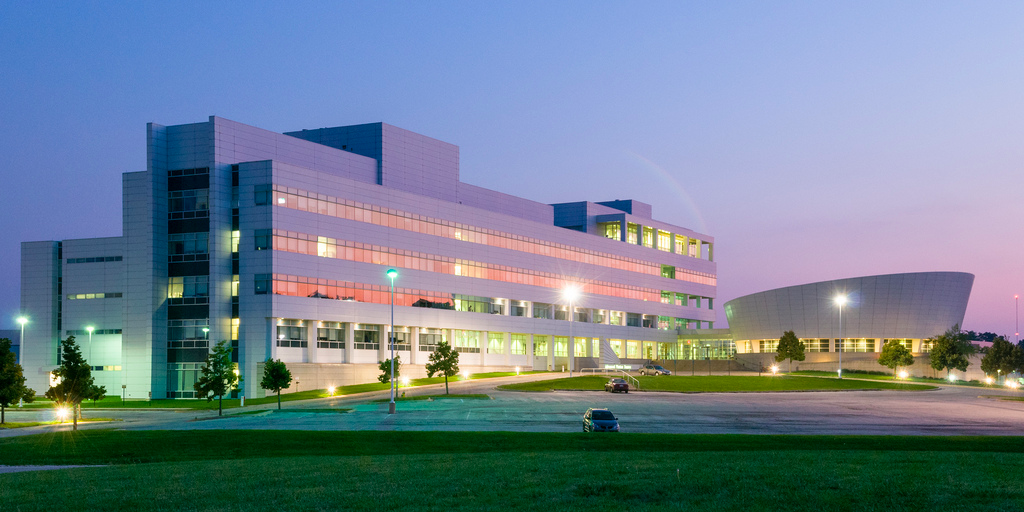
\includegraphics[width=\textwidth]{argonne.png}
	\captionof{figure}{Argonne National Laboratory}
\end{minipage}

\begin{minipage}{0.5\textwidth}
	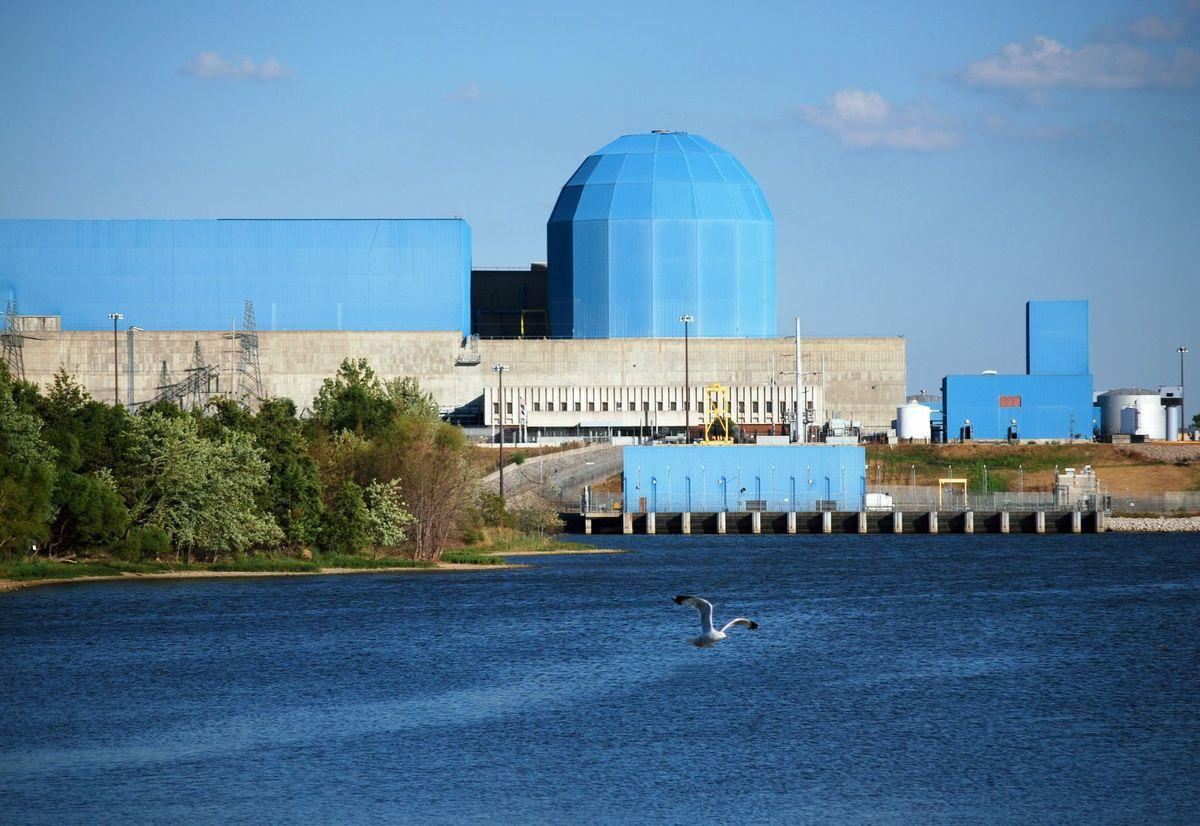
\includegraphics[width=\textwidth]{clintonpp.jpg}
	\captionof{figure}{Clinton Powerplant on Clinton Lake}
\end{minipage}
\begin{minipage}{0.5\textwidth}
	\textbf{Clinton Nuclear Power Plant}\\
Located about 35 miles away from Champaign, the Clinton Power Station is an Exelon owned nuclear power plant that started operating at full power on September 15th, 1987. They currently serve over one million customers and operate 94.9$\%$ of the time. The tour will be held on Thursday morning and bus transportation will be provided. Attendees will be guided by a Clinton employee. The tour will include the control-room simulator that operator trainees use, and a chance to learn more about the site’s innovative safety, operation, and engineering practices.
\end{minipage}

\begin{minipage}{0.5\textwidth}
	\textbf{National Pentascale Computing Facility (NPCF)}\\
Also located on campus is NCSA, which houses Blue Waters, one of the most powerful supercomputers in the world. The NCSA is within walking distance from all conference hotels. During the tour, attendees will tour the machine room and witness some of the beautiful results it produces. Supercomputers like Blue Waters are important for solving computationally challenging problems and creating robust simulations for a variety of phenomena.
\end{minipage}
\begin{minipage}{0.5\textwidth}
	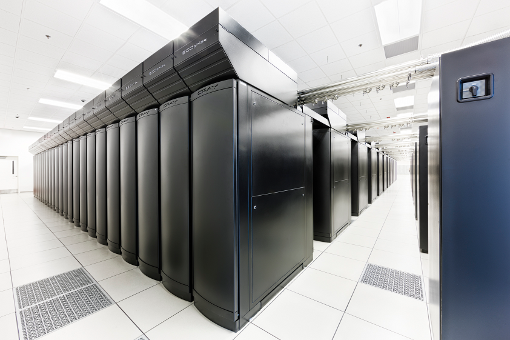
\includegraphics[width=\textwidth]{bw_front.png}
	\captionof{figure}{Blue Waters Supercomputer}
\end{minipage}

\textbf{Starfire Industries LLC}\\
Starfire Industries is located at the south end of campus and works with federal organizations such as DARPA, Homeland Security, NASA, and others. They offer services in areas like neutron radiography, fabrication, and prototyping. Students will be able to get to the site by using the MTD busses that run continuously throughout the day and will be free to all conference attendees. Here, students will be able to learn more about Starfire products such as the IMPULSE pulsed power module, plasma sources, thin film systems, nGen neutron generators, neutron detectors, and the PICTORIS neutron radiography system. Starfire’s collaboration with government agencies and propensity for solving big problems related to plasma engineering make them a great place to learn about plasma processing applications.\\


\subsubsection{Non-Technical Tours}



Brewery tours are staple social event and tour at the ANS Student Conference. Champaign-Urbana has several popular local breweries that give tours and tastings at their facilities. Due to this, we will be able to expand the number of attendees that can go on these tours over previous conferences. These will require sign up before the conference and we expect spots to fill up quickly.\\

\begin{minipage}{0.5\textwidth}
	% \centering
	\textbf{Riggs Brewery Tour}\\
For 21+ attendees, two tours of a local brewery will be included in our tours list Thursday afternoon from 3-5pm. Find out how Riggs makes their beer and taste test it along the way. Each tour will last approximately one hour and accommodates up to 20 people per tour. Riggs is located in east Urbana. Transportation to and from the brewery will be provided. 
\end{minipage}
\begin{minipage}{0.55\textwidth}
	\centering
	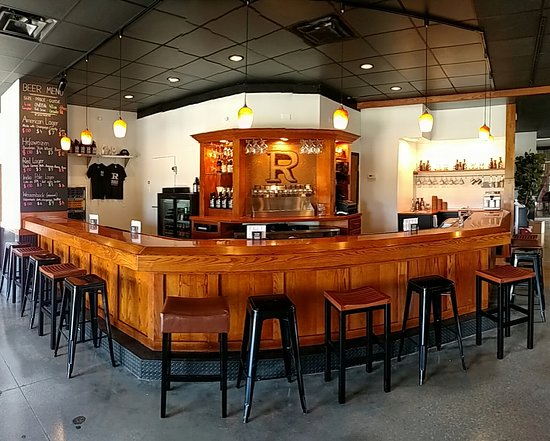
\includegraphics[width=0.75\textwidth]{riggs.jpg}
	\captionof{figure}{Riggs Brewery}
\end{minipage}

\begin{minipage}{0.5\textwidth}
	\centering
	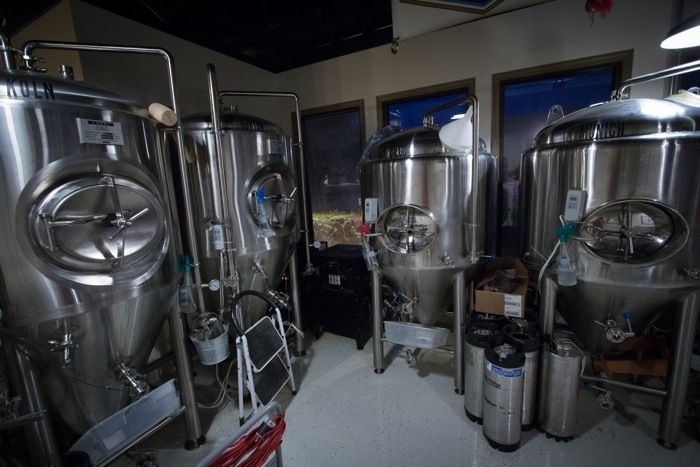
\includegraphics[width=0.75\textwidth]{triptych.jpeg}
	\captionof{figure}{Triptych Brewery Vessels -- Not RPVs}
\end{minipage}
\begin{minipage}{0.5\textwidth}
% \centering
	\textbf{Triptych Brewery Tour}\\
For 21+ attendees, Triptych offers two tours that run around 1.5 hours for roughly 30 people each that includes several beer tastings throughout. Tours will be from 2-5pm on Thursday afternoon. Triptych is located in Savoy, IL, just 15 minutes from campus. Transportation to and from the brewery will be provided.
\end{minipage}

\begin{minipage}{0.5\textwidth}
	\textbf{University Tour}\\
Attendees will be able to take a tour of the UIUC campus. They will start at the Talbot Laboratory where the department of Nuclear Plasma and Radiological Engineering is located. Here, students will get to see the Virtual Education and Research Laboratory to see how virtual reality technology can be adapted and applied to educational methods. There are also many other historical artifacts on display for participants to see. Afterwards, students will be led to various noteworthy locations unique to UIUC.
\end{minipage}
\begin{minipage}{0.5\textwidth}
	\centering
	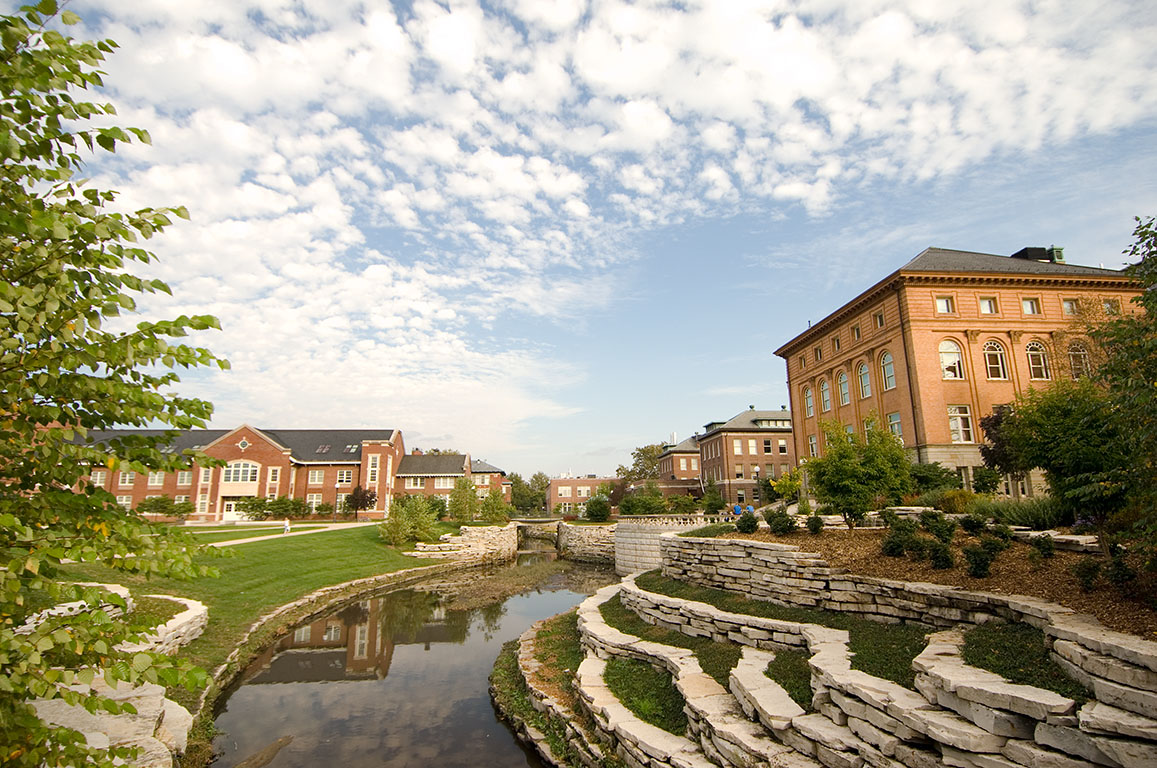
\includegraphics[width=0.75\textwidth]{creek.png}
	\captionof{figure}{Engineering Hall on the Beautiful Engineering Quad}
\end{minipage}
\\ 	


\subsection{Socials}

\subsubsection{Illini Union Rec Room Lockout}
The Illini Union Rec Room is located in the basement of the Union building. A Rec Room lockout gives ANS exclusive access to 14 bowling lanes, 12 billiard tables, and coin-operated arcade games following dinner at the Krannert Center for Performing Arts, only a short walk away through the University of Illinois main quad! This space can accompany up to 150 people, with extra tables outside of the Rec Room for socializing, playing board games, or having a late night snack or coffee with professionals or students from other universities.

% Illini Union Rec Room Picture
\begin{figure}[H]
	\centering
	\begin{subfigure}{0.5\textwidth}
		\centering
		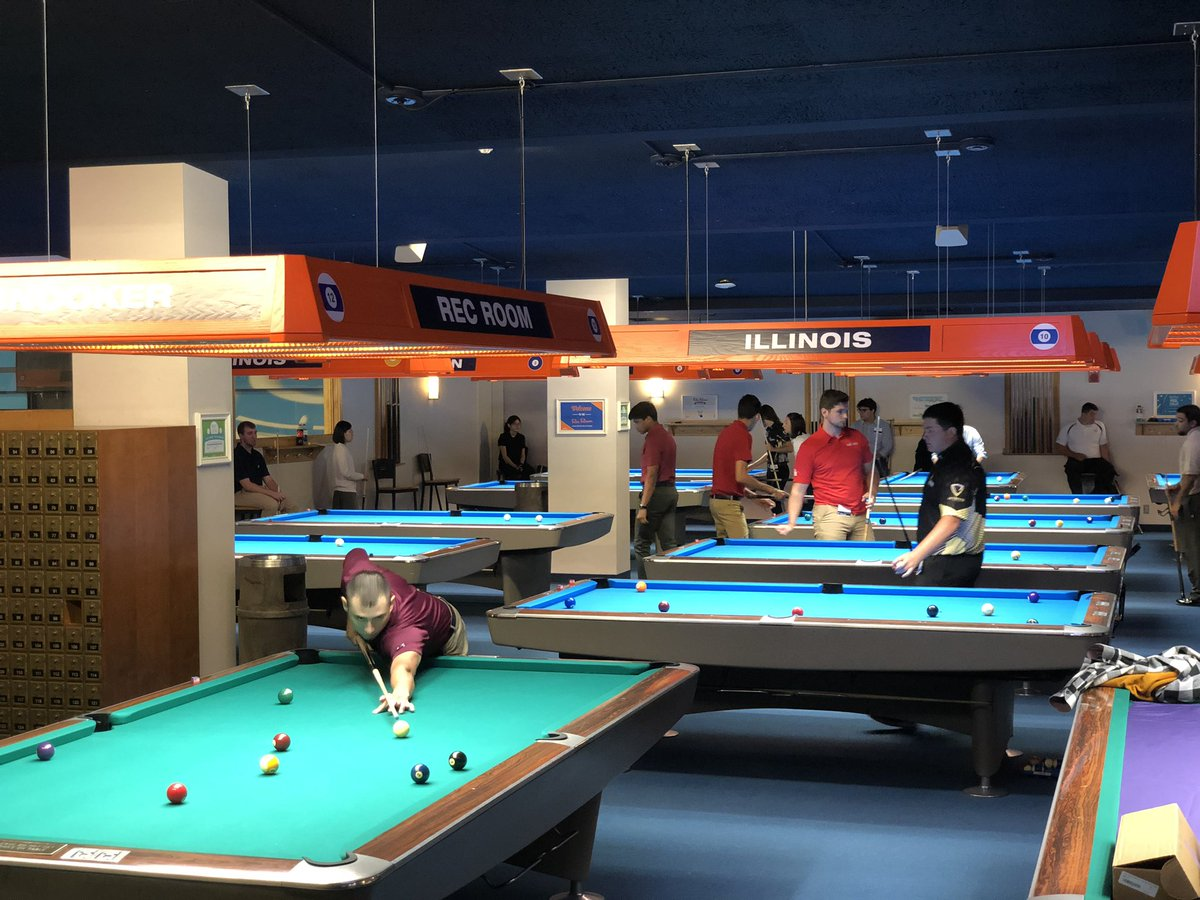
\includegraphics[width=0.9\linewidth]{union_recroom1.png}
	\end{subfigure}%
	\begin{subfigure}{0.5\textwidth}
		\centering
		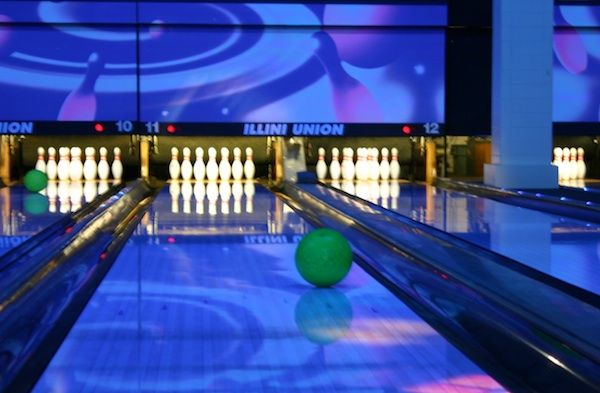
\includegraphics[width=0.9\linewidth]{union_recroom2.png}
	\end{subfigure}		
\end{figure} 

\subsubsection{77 Club at Memorial Stadium}
Memorial Stadium is not only home to the Fighting Illini football team, but also to exquisite event space overlooking Zuppke Field. The sixth level of Memorial Stadium is home of the magnificent 77 Club, which honors Illini great, the ``Galloping Ghost'' Red Grange. This 5,020 square foot space is located midfield and features an outdoor patio area overlooking the city of Champaign, for a combined total space of 9,740 square feet. This event will take place following dinner at I Hotel Conference Center, and is just a short and scenic walk away past the State Farm Center (formerly the historic Assembly Hall). Tables will be set up around a stage featuring live music and a dance floor and drinks will be served. This is the perfect event to incorporate a little bit of Illinois history with music, dancing, and socializing! 

% 77 Club Picture
\begin{figure}[H]
	\centering
	\begin{subfigure}{0.5\textwidth}
		\centering
		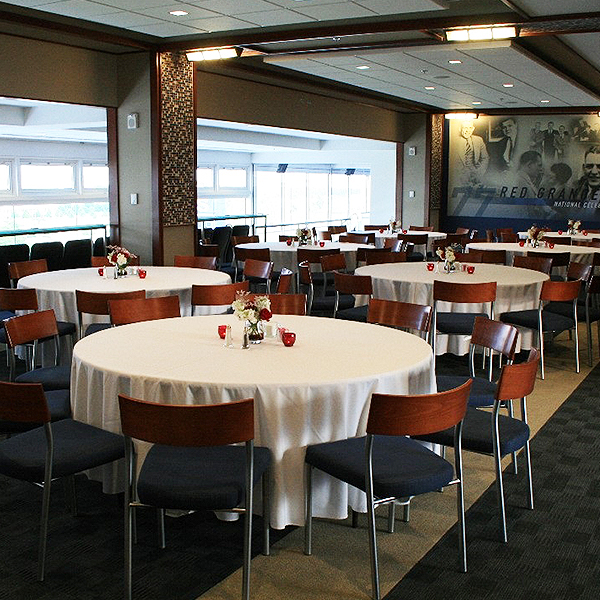
\includegraphics[width=0.7\linewidth]{77club1.png}
	\end{subfigure}%
	\begin{subfigure}{0.5\textwidth}
		\centering
		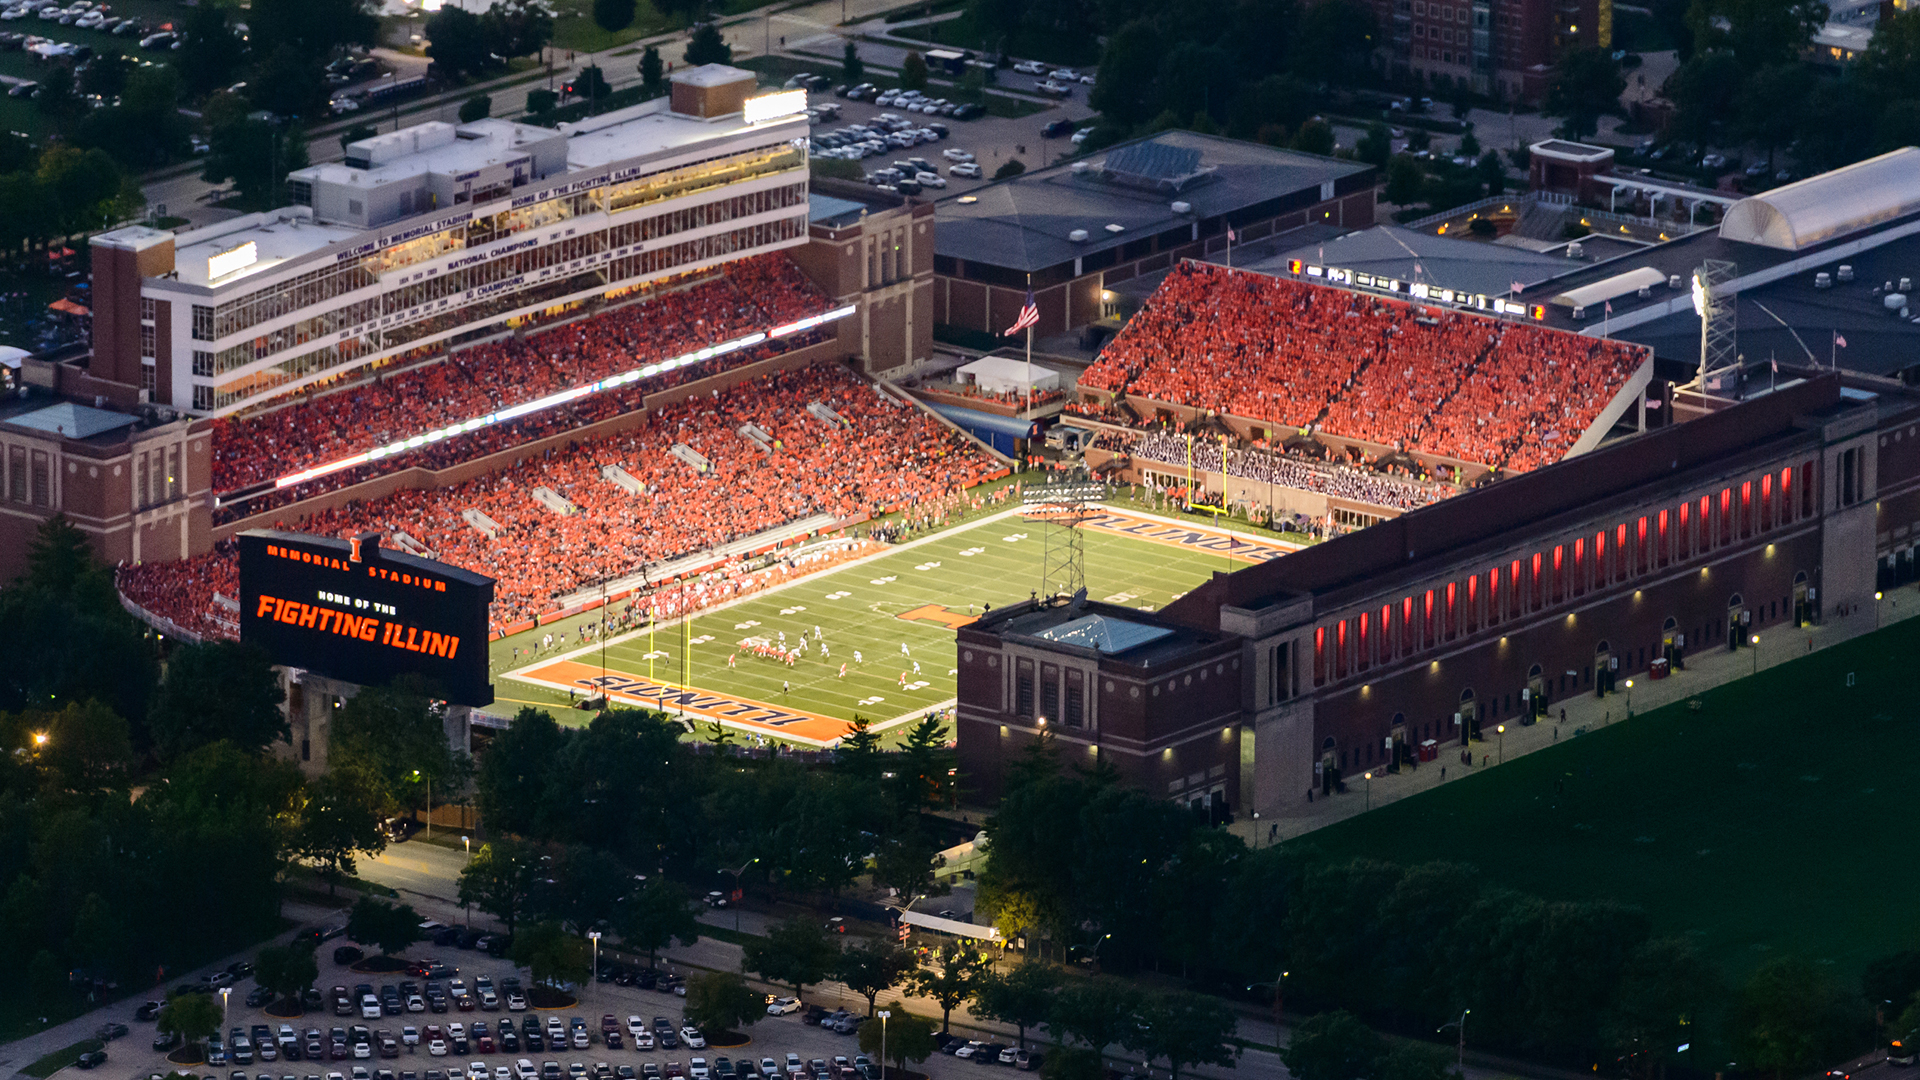
\includegraphics[width=0.9\linewidth]{77club2.png}
	\end{subfigure}		
\end{figure} 

\subsubsection{Pour Bros. Taproom in Downtown Champaign}
Welcome to Illinois' first pour-your-own taprooms. Pour Bros. Taproom is located in the heart of the historic downtown Champaign area and features 28 pour-your-own taps: beers, ciders, meads and wine\ldots all poured by you, one ounce at a time. Socialize over the vintage games Pour Bros has to offer: skeeball, bubble hockey, steel tip darts, DAGZ and more! If you are feeling more on the leisurely side, Pour Bros features live music in a spacious and comfortable seating area for you to get your networking on.

% Pour Bros Picture
\begin{figure}[H]
	\centering
	\begin{subfigure}{0.5\textwidth}
		\centering
		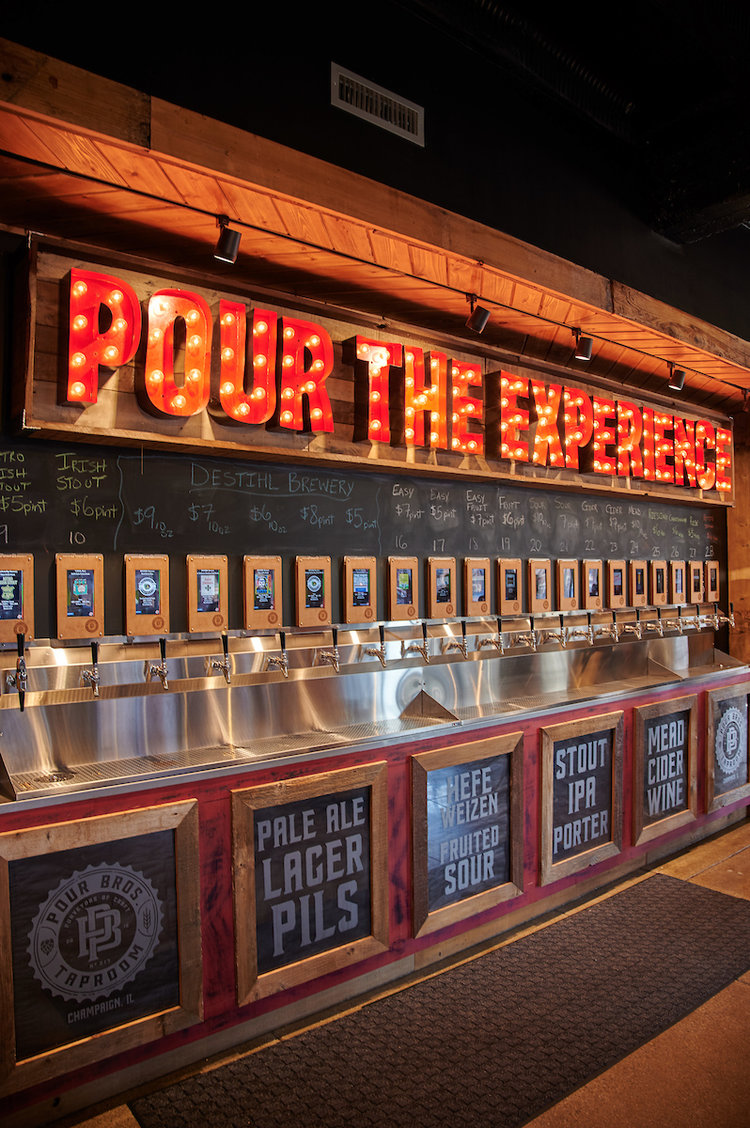
\includegraphics[width=0.5\linewidth]{pour_bros2.png}
	\end{subfigure}%
	\begin{subfigure}{0.5\textwidth}
		\centering
		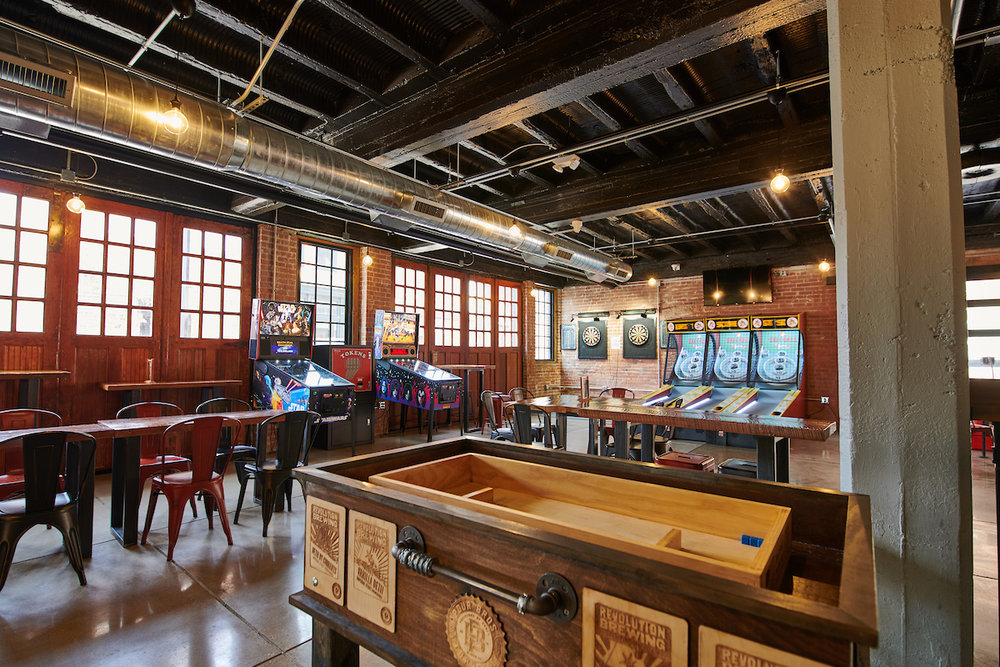
\includegraphics[width=0.9\linewidth]{pour_bros1.png}
	\end{subfigure}		
\end{figure} 

\subsubsection{Under 21 Social: University of Illinois Ice Arena}
For students under the drinking age that cannot attend the Pour Bros. Taproom social event, the University of Illinois Ice Arena is another option that is only a brief walking distance from the Union. It was built in 1931 and offers a unique option for skating get-togethers from broomball and hockey to group skating parties. The Ice Arena is a 55,000 square foot facility and is the only one in Champaign-Urbana. The dimensions of the rink are 192' by 115' with a 1,200 seat arena surrounding. There are four public locker rooms, four party areas, and two Zambonis in the facility. The Center Ice Cafe offers hot chocolate, coffee, smoothies, fountain drinks, and more to quench your thirst.  Snacks and concession items are also available.

% Ice Arena Picture
\begin{figure}[H]
	\centering
	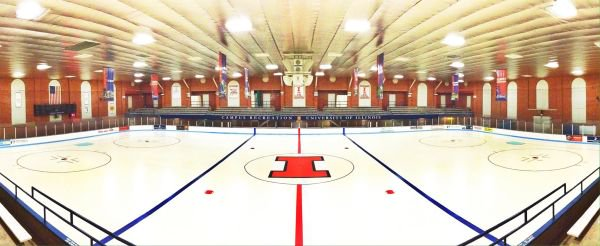
\includegraphics[width=0.8\textwidth]{ice_arena.png}
\end{figure}

